\documentclass[runningheads]{llncs}
%
\usepackage[T1]{fontenc}
% T1 fonts will be used to generate the final print and online PDFs,
% so please use T1 fonts in your manuscript whenever possible.
% Other font encodings may result in incorrect characters.
%
\usepackage{graphicx}
\usepackage{mathtools}

\newcommand{\M}{\mathcal{M}}


\usepackage[dvipsnames]{xcolor}
\definecolor{bluegray}{rgb}{0.5, 0.65, 0.85}
\definecolor{pastelgreen}{HTML}{58bc82}
\definecolor{greengray}{rgb}{0.5, 0.85, 0.65}
\definecolor{sandstone}{rgb}{0.8, 0.6, 0.2}
\definecolor{ruby}{HTML}{D81E5B}
\definecolor{teal}{HTML}{0E6C6B}
\definecolor{cyan}{HTML}{08B2E3}
\definecolor{purple}{HTML}{52489C}
\definecolor{scblue}{HTML}{1F73A9}
\definecolor{scgray}{HTML}{656A6D}
\definecolor{scred}{HTML}{DA2C38} % poppy

\usepackage[T1]{fontenc}
\usepackage{anyfontsize}
\usepackage{textcomp}
\usepackage[utf8x]{inputenc}

% fixes weird matplotlib for me that the others don't have
\def\mathdefault#1{#1}

\usepackage{amsmath}
\usepackage{amssymb}
\usepackage{thm-restate}
\usepackage{url}
\usepackage{csquotes}
\usepackage{longtable}

\usepackage{algpseudocode}

\usepackage{etoolbox}

\newenvironment{proofsketch}{\begin{proof}[Proof sketch]}{\end{proof}}

\makeatletter
\pretocmd{\thmt@rst@storecounters}{\Hy@SaveLastskip}{}{}
\apptocmd{\thmt@rst@storecounters}{\Hy@RestoreLastskip}{}{}
\makeatother


\usepackage{orcidlink}

\usepackage{algorithm}
\usepackage{algpseudocode}

\algrenewcommand\algorithmicrequire{\textbf{Input:}}
\algrenewcommand\algorithmicensure{\textbf{Output:}}

\usepackage{mdframed}

\usepackage{paralist}

\usepackage{graphicx}

\usepackage{adjustbox}
\usepackage{varwidth}

\usepackage{microtype}

\usepackage{stmaryrd}

\usepackage{nicefrac}
\usepackage{underscore}
\usepackage{booktabs}
\usepackage{wrapfig}
\usepackage{multirow, multicol}
\usepackage[table]{xcolor}

\usepackage{forest}
\usepackage{marvosym}

\usepackage[english]{babel}

\usepackage{cite}
\usepackage[capitalise]{cleveref}

\crefname{problem}{Problem}{Problems}
\crefname{definition}{Def.}{Defs.}
%\pagestyle{plain}

\renewcommand{\paragraph}[1]{\smallskip\noindent\emph{#1}~}
\renewcommand{\subsubsection}[1]{\medskip\noindent\textbf{#1}~}


%\usepackage{todonotes}
%\newcommand{\lin}[2][]{\todo[color=green!50, #1]{LH: #2}}
%\newcommand{\tq}[2][]{\todo[color=blue!50, #1]{TQ: #2}}
%\newcommand{\seb}[2][]{\todo[color=red!50, #1]{SJ: #2}}
%\newcommand{\sj}[2][]{\todo[color=red!50, #1]{SJ: #2}}
%\newcommand{\jpk}[2][]{\todo[color=yellow!50, #1]{JPK: #2}}

\usepackage{tikz, pgf, tikz-cd}
\usetikzlibrary{automata, positioning, shapes.geometric, shapes.symbols, patterns, fit, backgrounds}
\tikzset{elliptic state/.style={draw,ellipse}}
\tikzstyle{block} = [rectangle, draw,
    text width=2.5cm, text centered, rounded corners, minimum height=4em]
\tikzstyle{decision} = [diamond, draw,
    text width=1.5cm, text badly centered, inner sep=2pt]

\tikzset{every state/.style={inner sep=0pt, minimum size=15pt}}
\tikzset{pMC/.style={node distance=1.4cm, on grid, auto, initial text=,every label/.style={font=\footnotesize}}}

\usepackage{pgfplots}
\pgfplotsset{compat=newest}
\usepgfplotslibrary{groupplots}
\usepgfplotslibrary{polar}
\usepgfplotslibrary{statistics}
\usepgfplotslibrary{fillbetween}

\usepackage{pifont}
\newcommand{\cmark}{\ding{51}}%
\newcommand{\xmark}{\ding{55}}%
\newcommand{\yes}{\textcolor{pastelgreen}{\cmark}}
\newcommand{\no}{\textcolor{ruby}{\xmark}}
\newcommand{\dontmatter}{\textcolor{gray!80}{\textbf{?}}}


\usepackage{xspace}
\newcounter{goodsmileys}
\newcounter{badsmileys}
\newcommand{\OurSmiley}[2]{%
	\begin{tikzpicture}[-,scale=#2]
	\newcommand*{\SmileyRadius}{1.0}%
	%\draw [draw=none] (0,0) circle (\SmileyRadius)% outside circle
	%node [yshift=-0.22*\SmileyRadius cm] {\tiny #1}% uncomment this to see the smile factor
	
	% ogen
	\pgfmathsetmacro{\eyeX}{0.5*\SmileyRadius*cos(30)}
	\pgfmathsetmacro{\eyeY}{0.3*\SmileyRadius*sin(30)}
	\draw [line width=0.28mm] (\eyeX-0.25,\eyeY) -- (\eyeX-0.25,\eyeY+0.4);
	\draw [line width=0.28mm] (-\eyeX+0.25,\eyeY) -- (-\eyeX+0.25,\eyeY+0.4);
	
	% mond
	\pgfmathsetmacro{\xScale}{2*\eyeX/180}
	\pgfmathsetmacro{\yScale}{1.0*\eyeY}
	\draw[line width=0.28mm, domain=-\eyeX:\eyeX]
	plot ({\x},{
		-0.1+#1*0.15 % shift the smiley as smile decreases
		-#1*1.75*\yScale*(sin((\x+\eyeX)/\xScale))-\eyeY});
	\end{tikzpicture}%
}%
\newcommand{\good}{%
  \stepcounter{goodsmileys}%
  \OurSmiley{0.6}{0.22}\xspace%
}
\newcommand{\bad}{%
  \stepcounter{badsmileys}%
  \OurSmiley{-0.6}{0.22}\xspace%
}

\mdfdefinestyle{MyFrame}{%
    linecolor=black,
    outerlinewidth=0pt,
    innertopmargin=2pt,
    innerbottommargin=2pt,
    innerrightmargin=2pt,
    innerleftmargin=2pt,
    leftmargin = 2pt,
    rightmargin = 2pt
}

\usepackage{menukeys}

\newif\ifcamera
% \cameratrue          % camera-ready
\camerafalse       % full version
\newcommand{\appref}[2]{%
  \ifcamera
    App.~#2~\cite{arxiv}%
  \else
    App.~\ref{#1}%
  \fi
}

\newcommand{\Paths}{\mathrm{Paths}}
\newcommand{\FinPaths}{\mathrm{FinPaths}}
\newcommand{\Distr}{\Delta}
\newcommand{\Hist}{\mathrm{Hist}}
\newcommand{\THist}{\mathrm{THist}}
\newcommand{\Pre}{\mathrm{Prefix}}
\newcommand{\Allow}{\mathrm{Allow}}
\newcommand{\Live}{\mathrm{Live}}
\newcommand{\Dirac}{\mathbf{1}}

\usepackage{scalerel}
\newcommand\shieldbase{%
  \tikz[baseline=0.2ex] \draw[semithick]
    (0,1.75ex) -- (0,0.75ex)
    arc [radius=0.75ex, start angle=-180, end angle=0]
    -- (1.5ex,1.75ex) -- cycle;%
}
\DeclareRobustCommand\shield{%
  \mathord{\scalerel*{\shieldbase}{\bigcirc}}%
}

%old makros 
\newcommand{\ensuremathspace}[1]{\ensuremath{#1}\xspace}
\newcommand{\mathsymbol}[2]{ \newcommand{#1}{\ensuremathspace{#2}} }

\mathsymbol{\sinit}{s_{0}}
\mathsymbol{\Act}{\mathrm{Act}}
% \mathsymbol{\SafeAct}{\mathrm{SafeAct}}
\mathsymbol{\SafeAct}{\mathrm{Act^{Safe}}}
\mathsymbol{\act}{\alpha}
\mathsymbol{\mpm}{\mathcal{P}}
\mathsymbol{\mdp}{\mathcal{M}}
\mathsymbol{\mdpT}{(S,\sinit,\Act,\mpm)}
\mathsymbol{\mcT}{(S,\sinit,\mpm)}
\mathsymbol{\unitinterval}{[0,1]}
%\newcommand{\prob}[2][]{\mathbb{P}\left[ #1 \models #2\right ]}
\newcommand{\F}[1]{\diamond #1}

\newcommand{\sched}[1][]{\ensuremathspace{ \pi_{#1} }}
\mathsymbol{\schedopt}{\sched[]^{*}}
\newcommand{\schedulers}[1][M]{\Sigma^{#1}}
\mathsymbol{\imc}{\mdp^{\sched}}

\renewcommand{\Pr}{\mathrm{Pr}}

%\newcommand{\shield}{S}
\newcommand{\slack}{\mathit{slack}}
\newcommand{\guard}{\mathit{guard}}
\newcommand{\capacity}{\mathit{capacity}}
\newcommand{\hist}{\mathit{hist}}
\newcommand{\rrisk}{\mathit{rrisk}}
\newcommand{\hpath}{\mathit{path}}
\newcommand{\last}{\mathit{last}}
\newcommand{\choice}{\mathit{choice}}
\newcommand{\choices}{\mathit{choices}}
\newcommand{\supp}{\mathit{supp}}
\newcommand{\E}{\mathbb{E}}
%\newcommand{\Act}{\mathit{Act}}
\newcommand{\mix}{\mathit{mix}}
\newcommand{\itp}{\mathit{itp}}
\newcommand{\update}{\mathit{update}}
\newcommand{\rem}{\mathit{rem}}
\newcommand{\trunc}{\mathit{trunc}}
\newcommand{\T}{\mathcal{T}}
\newcommand{\Ht}{\mathcal{H}}
\newcommand{\Safe}{\mathrm{Safe}}
\newcommand{\Shields}{\mathrm{Shields}}

\mathsymbol{\shieldSafe}{\shield_{\Safe}}
\mathsymbol{\shieldDelta}{\shield_{\delta}}
\mathsymbol{\shieldDeltaPlus}{\shield_{\delta^+}}
\mathsymbol{\shieldOpt}{\shield_{\mathit{opt}}}
\mathsymbol{\shieldPess}{\shield_{\mathit{pess}}}
\mathsymbol{\shieldOnl}{\shield_{\mathit{onl}}}
\mathsymbol{\shieldOff}{\shield_{\mathit{off}}}
\mathsymbol{\shieldMemoryless}{\shield_{\mathit{ML}}}

\newcommand{\SafetyStrong}{\textbf{(S+)}\xspace}
\newcommand{\SafetyWeak}{{\textbf{(S\(-\))}\xspace}}
\newcommand{\PermissivenessStrong}{\textbf{(P+)}\xspace}
\newcommand{\PermissivenessWeak}{\textbf{(P\(-\))}\xspace}
\newcommand{\SaturatedPermisiveness}{\textbf{(P*)}\xspace}


\newcommand{\opt}{%
    \mathop{\mathrm{dir}}
}

% \usepackage{todonotes}
 \newcommand{\customcomment}[2]{\marginpar{\textcolor{#1}{\scriptsize{#2}}}}
 \newcommand{\lh}[1]{\customcomment{orange}{LH: #1}}
 \newcommand{\sj}[1]{\customcomment{red}{SJ: #1}}
 \newcommand{\fm}[1]{\customcomment{green}{FM: #1}}
 \newcommand{\ra}[1]{\customcomment{blue}{RA: #1}}
% %\newcommand{\ra}[1]{}
\newcommand{\mc}[1]{\customcomment{gray}{MC: #1}}
% \newcommand{\mc}[1]{\textcolor{red}{#1}}
% \newcommand{\mcc}[1]{\customcomment{gray}{MC: #1}}

% for EU logos
\newlength\myheight
\newlength\mydepth
\settototalheight\myheight{Xygp}
\settodepth\mydepth{Xygp}
\setlength\fboxsep{2pt}
\newcommand*\inlinegraphics[1]{%
  \settototalheight\myheight{Xygp}%
  \settodepth\mydepth{Xygp}%
  \raisebox{-0.5\mydepth}{\includegraphics[height=\myheight]{#1}}%
}

\let\proof\relax\let\endproof\relax
\usepackage{amsthm}


\begin{document}

\section{Introduction}

Black-box shielding (us) vs.\ safe RL (e.g. ProSh) are quite different problem statements!

\section{Preliminaries}

We assume that \(V_{\min}(s_0) \leq \nu\).

\begin{definition}[History]
A \emph{history} is a sequence
\(
    h \coloneq s_0 \, d_1 \, \alpha_1 \, s_1 \, d_2 \, \alpha_2 \, \cdots \, s_t
\) such that \(s_0 \alpha_1 s_1 \alpha_2 \cdots s_t\) is a path, and for all \(0 \leq k < t\): \(d_{k+1} \in \Distr(\Act(s_k))\). 
Given a history \(h= s_0 d_1 \alpha_1 s_1 \cdots s_t\),
\begin{compactitem}
    \item \(\last(h) \coloneq s_t\)  is the last state of the history,
    \item \(\hpath(h) \coloneq s_0 \alpha_1 s_1 \cdots s_t\) is the path of the history,
    \item \(\choice(h, k) \coloneq d_{k}\) is the \(k\)-th history choice for \(1 \leq k \leq t\),
    \item \(h|_k \coloneq s_0 \, d_1 \, \alpha_1 \, \cdots s_k\) is the history prefix up to step \(k\) for \(0 \leq k \leq t\).
\end{compactitem}
\end{definition}

History \(h\) is \emph{consistent} with policy \(\pi\) if for all \(k\): \(\choice(h,k) = \pi(\hpath(h|_{k-1}))\).


\begin{definition}[Shield]
    A \emph{shield} is a function \(\shield: \Hist(\M) \times \Distr(\Act) \rightarrow \Distr(\Act)\).
\end{definition}

\begin{definition}[Policy Transformer of a Shield]
    \label{def:policytransformer}
    Given a shield \(\shield\), its policy transformer is the function \(\T_{\shield} : \Pi_{\M} \rightarrow \Pi_{\M}\) defined recursively by
    \begin{align*}
        \T_{\shield}(\pi)(s_0 \alpha_1 s_1 \cdots \alpha_t s_t) \coloneq\;& \shield(h_t, \pi(s_0 \alpha_1 s_1 \cdots \alpha_t s_t)),\\
        \text{where } h_t \coloneq\;& s_0 \; \T_{\shield}(\pi)(s_0) \; \alpha_1 \; s_1 \; \T_{\shield}(\pi)(s_0\alpha_1s_1) \; \alpha_2 \; \cdots \; \alpha_t \; s_t.
    \end{align*}
\end{definition}
A shield \(\shield\) \emph{allows} a policy \(\pi\) if \(\T_{\shield}(\pi) = \pi\). We write \(\Allow(\shield) = \{\pi \in \Pi_\M \mid \T_{\shield}(\pi) = \pi\}\) as the set of allowed policies of \(\shield\).
% A shield \(\shield\) is \emph{canonical} if (1) for all \(h \in \Hist(\M), d \in \Distr(\Act)\): \(\shield(h, d) \in \{d, d|_{\SafeAct(\last(h))}\}\), and (2) for all \(h\) not consistent with a policy in \(\Allow(\shield)\), \(\shield(h,d)=d|_{\SafeAct(\last(h))}\).


We consider the following \emph{guarantees} from \cite{DBLP:conf/cav/HeckMACJ26}:

\begin{mdframed}[style=MyFrame,nobreak=true]
Let $\M$ be an MDP and $\shield$ a shield.\\
\textbf{(S+): Strong Safety.} \(\T_{\shield}(\Pi_\M) \subseteq \Safe(\Pi_\M)\). \\
\textbf{(P*): Saturated Permissiveness.} For all \(\pi \in \Pi_\M \setminus \Allow(\shield)\), there is no shield \(\shield'\) satisfying \SafetyStrong such that \(\Allow(\shield) \cup \{\pi\} \subseteq \Allow(\shield')\).
\end{mdframed}
We call a shield \emph{safe} if it satisfies \SafetyStrong and \emph{saturated} if it satisfies \SafetyStrong and \SaturatedPermisiveness.

\section{Problem Statement}


All proofs are in \cref{app:proofs}.

\section{Risk allocation shields}


\begin{figure}[t]
    \begin{center}
        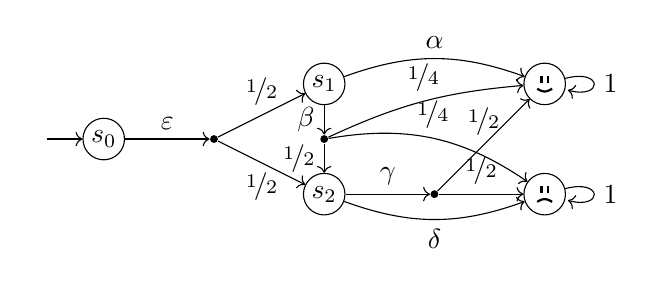
\begin{tikzpicture}[pMC]
            \node[state, initial left] (s0) {$s_0$};
            \node[circle, fill, inner sep=1pt] (eps) [right of=s0] {};
            \node[state] (s1) [right of=eps,yshift=0.7cm] {$s_1$};
            \node[state] (s2) [right of=eps,yshift=-0.7cm] {$s_2$};
            \node[] (s1b) [right of=s1] {};
            \node[circle, fill, inner sep=1pt] (s1mid) [right of=eps] {};
            \node[circle, fill, inner sep=1pt] (s2b) [right of=s2] {};
            \node[state] (good) [right of=s1b] {$\good$};
            \node[state] (bad) [right of=s2b] {$\bad$};
            \path[->] (s0) edge node[above] {$\varepsilon$} (eps);
            \path[->] (eps) edge node[below] {$\nicefrac{1}{2}$} (s2);
            \path[->] (eps) edge node[above] {$\nicefrac{1}{2}$} (s1);
            \path[->] (s1) edge[bend left=20] node[above] {$\alpha$} (good);
            \path[->] (s1) edge[] node[left] {$\beta$} (s1mid);
            \path[->] (s1mid) edge[] node[left] {$\nicefrac{1}{2}$} (s2);
            \path[->] (s1mid) edge[bend left=10] node[above] {$\nicefrac{1}{4}$} (good);
            \path[->] (s1mid) edge[bend left=22] node[above] {$\nicefrac{1}{4}$} (bad);
            \path[->] (s2) edge[] node[above] {$\gamma$} (s2b);
            \path[->] (s2b) edge[] node[above] {$\nicefrac{1}{2}$} (bad);
            \path[->] (s2b) edge[] node[above] {$\nicefrac{1}{2}$} (good);
            \path[->] (s2) edge[bend right=20] node[below] {$\delta$} (bad);
            \path[->] (bad) edge[loop right] node[right] {$1$} (bad);
            \path[->] (good) edge[loop right] node[right] {$1$} (good);
        \end{tikzpicture}
        \caption{Example MDP}
        \label{fig:mdpex}
    \end{center}
\end{figure}


Our goal is to build shields that behave as permissive as possible for the agents while preserving the strong safety guarantee \SafetyStrong. However, in general, there exists no single safe probabilistic shield that allows all safe agent behavior \cite{DBLP:conf/cav/HeckMACJ26}. This motivates that probabilistic shields should be tailored to an agent's behavior to be most effective.

For example, consider the MDP in \cref{fig:mdpex}: if the agent tends to play the safe action \(\alpha\) in \(s_1\) but takes a lot of risk in \(s_2\), a safe shield can block the action \(\beta\) in \(s_1\) in order to allow riskier choices in \(s_2\). The total amount of risk the agent can take is then \(r_{s_0} = \nicefrac{1}{2} \cdot r_{s_1} + \nicefrac{1}{2} \cdot r_{s_2}\), where \(r_{s_1}\) and \(r_{s_2}\) are the amount of risk allocated to \(s_1\) and \(s_2\), respectively. For the shield to be safe, \(r_{s_0}\) should be bounded by \(\nu\). The shield should thus have a selection rule with which to distribute the available risk between \(s_1\) and \(s_2\). This is what we call a \emph{risk allocation:}

\begin{definition}[Risk allocation]
    A \emph{risk allocation} is a function \(b : \Hist(\M) \times \Distr(\Act) \rightarrow \Distr(\Act \times S)\) such that for all \(h \in \Hist(\M)\) and \(d \in \Distr(\Act)\), we have that \(\supp(b(h,d)) \subseteq \{(\alpha, s') \mid d(\alpha) P(\last(h),\alpha,s') > 0\}\).
\end{definition}

Given a risk allocation, one can compute the amount of risk budget available at each history. This is the \emph{remaining risk budget.}

At \(s_0\), the remaining risk budget is the minimum of the risk threshold \(\nu\) and the worst-case risk in the MDP.

At each history \(h\), we recursively define the risk budget for every successor history \(h d \alpha s'\). First, the \emph{slack} for each choice \(d\) is the amount of risk that can still be allocated additionally to \(V_{\min}\), which depends on the remaining risk at \(h\). The outcome of playing \(d\) is that an action \(\alpha\) and a successor state \(s'\) will be sampled. We allocate some fraction of the slack using the risk allocation \(b(h,d)(\alpha,s')\), and then divide the result by the probability that this actually happens, which is \(d(\alpha) \cdot P(\last(h), \alpha, s')\). In the case that the choice exceeds the remaining budget or the outcome has probability zero, we simply allocate \(V_{\max}(s')\).

\begin{definition}[Remaining risk budget]
    \label{def:remainingrisk}
    Given a risk allocation \(b\), define the \emph{remaining risk budget} \(\rrisk_b: \Hist(\M) \rightarrow \mathbb{R}_{\geq 0}\) as follows. We set
    \begin{align*}
        \rrisk_b(s_0) &= \min \{ \nu, V_{\max}(s_0) \}, \\
        \rrisk_b(h d \alpha s') &=
        \begin{cases}
            V_{\min}(s') + \frac{\slack_b(h, d) \cdot b(h,d)(\alpha,s')}{d(\alpha) \cdot P(\last(h),\alpha,s')} &\text{if } \guard(h,d,\alpha,s'), \\
            V_{\max}(s') &\text{otherwise.}
        \end{cases} \\
        \text{where } \slack_b(h, d) &=  \min\{\rrisk_b(h), Q_{\max}(\last(h),d)\} - Q_{\min}(\last(h),d) \\
        \text{and } \guard(h,d,\alpha,s') &\Leftrightarrow Q_{\min}(\last(h),d) \leq \rrisk_b(h) \land d(\alpha)P(\last(h),\alpha,s') > 0.
    \end{align*}
\end{definition}

Finally, we define the shield \(\shield_b\) from budget allocation \(b\). It allows any choice as long as its achievable risk after each choice does not exceed the remaining risk induced by \(b\). If a choice cannot be allowed, we project to the closest allowed choice using a given distribution distance \(D\).

\begin{definition}[Shield from allocation]
\label{def:shield}
    Given a risk allocation \(b\) and a distance on distributions \(D\), the shield \(\shield_b\) is given as
    \begin{align*}
        \shield_b(h,d) &\coloneq \mathop{\mathrm{argmin}}_{d ' \in \mathcal{F}_b(h)} D(d, d'), \\
        \text{where } \mathcal{F}_b(h) &\coloneq \{d' \in \Distr(\Act(\last(h))) \mid Q_{\min}(\last(h), d') \leq \rrisk_b(h) \}.
    \end{align*}
\end{definition}



% \lh{Actually, we will still play ActSafe after a block, just not including the block itself!}

The next theorem states that whatever the risk allocation \(b\), the resulting shield \(\shield_b\) is safe. We provide a proof sketch, the full proof is given in \cref{app:proofs}.

\begin{theorem}
    \label{thm:allocationshieldsafe}
    For any risk allocation \(b\), the shield \(\shield_b\) is safe, i.e., satisfies \SafetyStrong.
\end{theorem}

\begin{proofsketch}
    Given any risk allocation \(b\), the remaining risk \(\rrisk_b\) is a nonnegative supermartingale, which is pointwise above the probability to reach \(\bad\). As the Q-values of any policy shielded using \(\shield_b\) are below \(\rrisk_b\), the expectation to reach \(\bad\) from \(s_0\) is thus less than \(\rrisk_b(s_0) \leq \nu\).
\end{proofsketch}


\section{Wasteless allocations and Saturation}

\begin{definition}[Wasteless risk allocation]
    A risk allocation \(b\) is \emph{wasteless} if for all histories \(h d \alpha s' \in \Hist(\M)\), we have \(
        \rrisk_b(h d \alpha s') \leq V_{\max}(s').
    \)
    
    % or, equivalently,
    % \[
    % b(h,d)(\alpha,s') \slack_b(h,d) \leq d(\alpha) P(\last(h),\alpha,s') (V_{\max}(s') - V_{\min}(s')).
    % \]
\end{definition}

\begin{example}
    Consider the MDP in \cref{fig:mdpex}, \(\nu = \nicefrac{2}{3}\), and a risk allocation \(b\) with \(b(s_0, \Dirac_\varepsilon) = \{\Dirac_{(\varepsilon, s_2)}\}\).
    Then we have:
    \begin{align*}
        \rrisk_b(s_0) &= \min \{\nicefrac{2}{3}, \nicefrac{7}{8}\} = \nicefrac{2}{3}, \\
        \rrisk_b(s_0 \Dirac_{\varepsilon} \varepsilon s_1) &= 0 + \frac{0 \cdot \nicefrac{5}{12}}{\nicefrac{1}{2}} = 0, \\
        \rrisk_b(s_0 \Dirac_{\varepsilon} \varepsilon s_2) &= \nicefrac{1}{2} + \frac{1 \cdot \nicefrac{5}{12}}{\nicefrac{1}{2}} = \nicefrac{4}{3} > 1.
    \end{align*}
    Thus, \(b\) is \emph{not} wasteless. Intuitively, \(s_2\) is assigned too much risk allocation under \(b\); that risk allocation could have been moved to \(s_1\).
\end{example}



\begin{theorem}
    \label{thm:wastlesssaturated}
    For any safe shield \(\shield\), there exists a wasteless risk allocation \(b\) such that \(\Allow(\shield_b) = \Allow(\shield)\) if and only if \(\shield\) is saturated.
\end{theorem}

% \begin{definition}[Wasteless Refinement]
%     Given a risk allocation \(b\), we call \(b^*\) a \emph{wasteless refinement} of \(b\) if (1) \(b^*\) is wasteless, and (2) \(\Allow(\shield_b) \subseteq \Allow(\shield_{b^*})\).
% \end{definition}

We now describe a simple algorithm to make a given risk allocation wasteless.
Given a risk allocation \(b\), suppose that \(b\) is already wasteless on all prefixes of a given history \(h\).
We define the \emph{allocation capacity}.
\begin{definition}[Allocation Capacity]
    \label{def:capacity}
    For a history \(h\) and choice \(d\), we define the \emph{allocation capacity} \(\capacity: S \times \Distr(\Act) \times \mathbb{R}_{\geq 0} \rightarrow \mathbb{R}_{\geq 0}^{S \times \Act}\) as \[
        \capacity(s, d, r)(\alpha, s') \coloneq 
        \begin{cases}
            \frac{d(\alpha) P(s,\alpha,s') (V_{\max}(s') - V_{\min}(s'))}{\min \{r, Q_{\max}(s, d)\} - Q_{\min}(s,d)} &\text{if defined and positive}, \\
            [d(\alpha) P(s,\alpha,s') > 0] &\text{otherwise.}
        \end{cases}
    \]
\end{definition}

We can then restate wastelessness in terms of capacity:

\begin{lemma}
    A risk allocation \(b\) is wasteless iff for all \(h \in \Hist(\M)\) and \(d \in \Distr(\Act)\), we have that \(b(h,d) \leq \capacity(\last(h),d, \rrisk_b(h))\) pointwise.
\end{lemma}

\begin{algorithm}[t]
    \caption{Make an allocation wasteless}
    \label{alg:makewasteless}
    \textbf{Input:} Allocation \(a \in \Distr(\Act \times S)\), local capacity \(c \in \mathbb{R}_{\geq 0}^{\Act \times S}\),  \\
    \textbf{Output:} Wasteless allocation \(a^* \in \Distr(\Act \times S)\)
    \begin{algorithmic}
    \Function{MakeWasteless}{$a,c$}
    \State \(a^\star \gets \min(a, c)\) \Comment{Pointwise minimum}
    \ForAll{\((\alpha,s') \in \Act \times S\)}
        \State \(a^\star(\alpha,s') \gets a^\star(\alpha,s')+ \min\{1-\lVert a^\star\rVert_1,\; c(\alpha,s')-a^\star(\alpha,s') \}\)
    \EndFor
    \State \Return \(a^\star\)
    \EndFunction
    \end{algorithmic}
\end{algorithm}

The algorithm in \cref{alg:makewasteless} describes how to make a risk allocation wasteless. We then define the \emph{wasteless refinement} of \(b\) as the recursive application of this algorithm:

\begin{definition}[Wasteless Refinement]
    A risk allocation \(b^*\) is a \emph{wasteless refinement} of \(b\)
    if \(b^*\) is wasteless and
    \(
        \Allow(\shield_b) \subseteq \Allow(\shield_{b^*}).
    \)
\end{definition}

\begin{theorem}
    \label{thm:wasteless}
    For risk allocation \(b\), the risk allocation \(b^*\) recursively defined as \[
        b^*(h,d) \coloneq \textsc{MakeWasteless}(b(h,d), \capacity(\last(h), d, \rrisk_{b^*}(h)))
    \] (\cref{alg:makewasteless}) is a wasteless refinement of \(b\).
\end{theorem}

\begin{theorem}
    \label{thm:allowablepolicy}
    For every safe policy \(\pi\), define the risk allocation \(b\) given by
    \[
        b(h,d)(\alpha,s') = \begin{cases}
            d(\alpha) P(s,\alpha,s') \frac{V^\pi(\hpath(h) \alpha s') - V_{\min}(s')}{V^\pi(\hpath(h)) - Q_{\min}(s,d)} &\text{if } d = \pi(\hpath(h)) \\ &\text{and } V^\pi(s) > Q_{\min}(s,d), \\
            d(\alpha) P(s,\alpha,s') &\text{otherwise.}
        \end{cases}
    \]
    For the wasteless refinement \(b^*\) of \(b\), we have \(\pi \in \Allow(\shield_{b^*})\).%, and \(\shield_{b^*}\) is saturated.
\end{theorem}

\begin{corollary}
    For every safe \emph{memoryless} policy \(\pi\), there exists a \emph{memoryless} risk allocation \(b: S \times \Distr(\Act) \rightarrow \Distr(\Act \times S)\) such that we have \(\pi \in \Allow(\shield_{b})\).%, and \(\shield_{b^*}\) is saturated.
\end{corollary}

\begin{remark}
    By taking a wasteless refinement of \(b\), one can even construct a saturated shield allowing \(\pi\).
\end{remark}


% \begin{figure}[t]
%     \centering
%     \begin{forest}
%     for tree={
%         edge={->},
%         where n=1
%             {edge label={node[auto,pos=1,swap]{Yes}}}
%             {edge label={node[auto,pos=1]{No}}},
%     },%[\(V^\pi\) available and \(V^\pi(s_0)\leq\nu\)?
%         %[ Solve exactly (\cref{thm:allowablepolicy})]
%     [ Access to agent oracle and env/simulator?
%         [ Use \emph{online} learning ]
%         [ Access to execution logs?
%             [ Use \emph{offline} learning ]
%             [ Use generic shield ]
%         ]
%     ]
%     %]
%     \end{forest}
%     \caption{When to use online and offline learning.}
%     \label{fig:onlineoffline}
% \end{figure}

% \begin{figure}[t]
%     \centering
%     \input{shield-learning.tex}
%     \caption{Offline and online learning of a shield.}
%     \label{fig:shield-learning}
% \end{figure}

\section{Online Learning of Shield}

To learn a shield online, we first have to define an objective to optimize towards. We define the \emph{intervention cost} as the.

\begin{definition}[Intervention cost]
    The \emph{(discounted) intervention cost} of policy \(\pi\) under risk allocation \(b\) for discount factor \(\gamma \in (0,1]\) is defined as
    \[
    J_\gamma(b; \pi) \coloneq \E_{\tau \sim \T_{\shield_b}(\pi)} \left(
        \sum_{t \geq 0} \gamma^t D(\pi(\tau|_t), \T_{\shield_b}(\pi)(\tau|_t))
    \right).
    \]
\end{definition}

\begin{definition}[Allowed steps]
    The \emph{(discounted) allowed steps} of policy \(\pi\) under risk allocation \(b\) for discount factor \(\gamma \in (0,1]\) is defined as
    \[
    T_\gamma(b; \pi) \coloneq \E_{\tau \sim \T_{\shield_b}(\pi)} \left(
        \sum_{t \geq 0} \gamma^t [\pi(\tau|_t')=\T_{\shield_b}(\pi)(\tau|_{t'}) \text{ for all }  0 \leq t' \leq t]
    \right).
    \]
\end{definition}

\lh{Optimize time until first block? \(\gamma^t\) where \(t\) is time of first block, 0 if no block occurs}

\begin{algorithm}[t]
    \begin{algorithmic}
        \State \(h \gets s_0\) \Comment{Current history}
        \State \(r \gets \min \{\nu, V_{\max}(s_0)\}\) \Comment{Remaining risk budget}
        \State \(\widehat{J} \gets 0\) \Comment{Intervention cost}
        \For{\(t \in \{0, \ldots, T-1\}\)}
            \Statex \emph{Invariant:} \(r = \rrisk_{b_\theta^*}(h)\)
            \State \(d_A \gets \textsc{Agent}(\hpath(h))\) \Comment{Get agent's choice}
            \State \(d \gets \shield_{b^*_{\theta}}(h, d_A)\) \Comment{Apply shield (\cref{def:shield}) using \(r = \rrisk_{b_\theta^*}(h)\)}
            \State \(b_{h,d} \gets b_{\theta}(h,d)\) \Comment{Evaluate parametrized allocation}
            \State \(c \gets \capacity(\last(h),d, r)\) \Comment{Compute capacity (\cref{def:capacity})}
            \State \(b_{h,d} \gets \textsc{MakeWasteless}(b_{h,d}, c)\) \Comment{Get wasteless risk allocation (\cref{alg:makewasteless})}
            \Statex \emph{Invariant:} \(b_{\theta}^*(h,d) = b_{h,d}\)
            \State Sample \(\alpha \sim d\) \Comment{Execute choice}
            \State Sample \(s' \sim P(\last(h),\alpha,\cdot)\) \Comment{Make a step}
            \State \(r \gets \rrisk_{b_\theta^*}(h d \alpha s')\) \Comment{One recursive risk step (\cref{def:remainingrisk}}) using \(r\) and \(b_{h,d}\)
            \State \(h \gets h d \alpha s'\); \; \(\widehat{J} \gets \widehat{J} + \gamma^t D(d_A,d)\) \Comment{Update history and intervention cost}
        \EndFor
        \State \Return \(\widehat{J}\)
    \end{algorithmic}
    \caption{Executing an epsidode with the allocation shield}
\end{algorithm}

\bibliographystyle{splncs04}
\bibliography{literature}

\ifcamera

\else
\newpage
\appendix
\begingroup



\section{Proofs}
\label{app:proofs}

\subsection{Proof of \cref{thm:allocationshieldsafe}}
\begin{proof}
    Let \(\pi \in \Pi(\M)\). We show that \(\pi' \coloneq \T_{\shield_b}(\pi)\) is safe. We show that for all \(t \in \mathbb{N}\), we have \(\Pr^{\pi'}(s_0 \vDash \diamond^{\leq t} \bad) \leq \nu\), which implies that  \(V_{\pi'}(s_0 ) \leq \nu\). Because \(\pi\) was arbitary, this shows safety of \(\shield_b\).

    Consider the stochastic process on histories \(H_t\) generated by executing \(\pi'\) in \(\M\) in \(t\) steps. Let \(d \coloneq \pi'(\hpath(h))\) and \(s \coloneq \last(h)\). We then have
    \begin{align*}
        & \E\left[\rrisk_b(H_{t+1}) \mid H_t = h\right] \\
        &= \sum_{\substack{\alpha, s' \\ d(\alpha)P(s,\alpha,s')>0}} d(\alpha) P(s,\alpha,s') \rrisk_b(h d  \alpha s') \\
        &\overset{(\star)}{=}\sum_{\substack{\alpha, s' \\ d(\alpha)P(s,\alpha,s')>0}} d(\alpha) P(s,\alpha,s')  \left( V_{\min}(s') + \frac{b(h,d)(\alpha,s') \cdot \slack_b(h, d)}{d(\alpha) \cdot P(s,\alpha,s')} \right)  \\
        &= Q_{\min}(s,d) +   \slack_b(h,d) \underbrace{\sum_{\alpha, s'} b(h,d)(\alpha,s')}_{=1} \\
        &= \min \{ \rrisk_b(h), Q_{\max}(s,d) \} \\
        &\leq \rrisk_b(h).
    \end{align*}
    Here, \((\star)\) follows from the fact that \(d = \pi'(\hpath(h)) = \shield_b(h, \pi(\hpath(h))) \in \mathcal{F}_b(h)\), we have \(Q_{\min}(\last(h), d) \leq \rrisk_b(h)\).
    Moreover, \(\rrisk_b(h) \geq V_{\min}(\last(h)) \geq 0\). Thus, \(\rrisk_b\) is a nonnegative supermartingale.
    Using the stochastic process \(H_t\), define another stochastic process \[
        X_t \coloneq \begin{cases}
            1 &\text{if } H_t \text{ contains } \bad, \\
            0 &\text{otherwise}.
        \end{cases}
    \]
    We have that \(\Pr^{\pi'}(s_0 \vDash \diamond^{\leq t} \bad) = \E[X_t]\) by definition of reachability.
    Moreover, we have that \(X_t \leq \rrisk_b(H_t)\), as \(\bad\) is absorbing. Thus, taking expectations of the latter equation and using the supermartingale property gives
    \[
        \Pr^{\pi'}(s_0 \vDash \diamond^{\leq t} \bad) \leq
        \E[\rrisk_b(H_t)] \leq \E[\rrisk_b(H_0)] = \rrisk_b(s_0) \leq \nu.
    \]
    We have thus shown the required statement above, and thus, \(\shield_b\) is safe.
\end{proof}

\subsection{Proof of \cref{thm:wastlesssaturated}}

% We recall the definition  \emph{history mixing} and a lemma from \cite{DBLP:conf/cav/HeckMACJ26}:
% \begin{definition}[History Mixing]
%     Given a set of policies \(P\subseteq\Pi_\M\), the \emph{history mixing} is the set \(\mix(P)\subseteq\Pi_\M\) such that \(\pi \in \mix(P)\) if:
%     \[
%     \forall h \in \Hist(\M). \; h \text{ is consistent with } \pi \implies (\exists \pi' \in P. \; h \text{ is consistent with } \pi').
%     \]
% \end{definition}

% \begin{lemma}
%     \label{prop:mixclosed}%
%    Given shield~\(\shield\) and policies \(P \subseteq \Allow(\shield)\). Then \(\mix(P) \subseteq \Allow(\shield)\).
% \end{lemma}%


% \begin{definition}[Locally Allowed Choices]
%     Given shield \(\shield\), we define the \emph{locally allowed choices} \(A_{\shield}(h) : \Hist(\shield) \rightarrow \Distr(\Act)\) as
%     \[
%         A_{\shield}(h) \coloneq \{d \mid \exists \pi \in \Allow(\shield) \text{ s.t. } h \text{ consistent with } \pi \text{ and } \pi(\hpath(h))=d \}.
%     \]
% \end{definition}

% \begin{definition}[Worst Continuation Risk]
% \end{definition}

% \begin{definition}[Risk-tight]
%     We say that shield \(\shield\) is \emph{risk-tight} if the following hold for all \(h \in \Hist(\shield)\) and \(d \in \Distr(\Act)\):
%     \begin{align}
%         R_\shield(s_0) &= \min \{ \nu, V_{\max}(s_0) \} \tag{RT1}, \\
%         d \in A_{\shield}(h) &\iff Q_{\min}(\last(h),d) \leq R_{\shield}(h), \tag{RT2} \\
%         d \in A_{\shield}(h) \implies \sum_{\alpha,s'} d(\alpha) P(\last(h), \alpha, s') &= \min \{ R_{\shield}(h), Q_{\max}(\last(h),d))\}, \tag{RT3}, \\
        
%     \end{align}
% \end{definition}


\begin{proof}
    For a given shield \(\shield\), write
    \[
        \Hist(\shield)
        \coloneq
        \left\{
            h\in\Hist(\M)
            \mid
            \exists\pi\in\Allow(\shield):
            h\text{ is consistent with }\pi
        \right\}.
    \]
    Define \(R_{\shield} : \Hist(\shield) \rightarrow [0,1]\) as the worst case probability of reaching \(\bad\) starting at \(h\):
    \[
        R_{\shield}(h) = \sup_{\substack{\pi \in \Allow(\shield) \\ \pi \text{ consistent with } h}} V_{\pi}(\hpath(h)).
    \]
    Note that \(R_{\shield}(h)\) is a supermartingale for any stochastic process on histories \(H_t\) generated by executing a policy \(\pi \in \Allow(\shield)\) on \(\mathcal{M}\).

    \enquote{\(\Leftarrow\)}:
    Let \(\shield\) be a saturated shield.
    
    \paragraph{Proof that there exists a risk allocation \(b\) such that \(R_{\shield}(h) \leq \rrisk_b(h)\)}.
    We claim that there exists a risk allocation \(b\) such that \(R_{\shield}(h) \leq \rrisk_b(h)\) for all \(h \in \Hist(\shield)\), and \(b\) is wasteless.
    We construct this risk allocation inductively at each history \(h \in \Hist(\shield)\), maintaining the induction hypothesis
    \begin{align}
        R_{\shield}(h) \leq \rrisk_b(h) \leq V_{\max}(\last(h)). \label{eq:hypothesis}
    \end{align}
    Because \(\shield\) is safe, we have \(R_{\shield}(s_0) \leq \min \{\nu, V_{\max}(s_0)\} = \rrisk_b(s_0)\).
    For the induction step, suppose \cref{eq:hypothesis} holds for \(h\) and consider the history \(h d \alpha s'\).

    First, we have by \cref{eq:hypothesis} and the supermartingale property of \(R_{\shield}\):
    \begin{align*}
        \sum_{\alpha, s'} d(\alpha) P(\last(h), \alpha, s') R_{\shield}(h d \alpha s') \leq R_{\shield}(h) \leq  \rrisk_b(h).
    \end{align*}
    
    Next, we have by definition of \(R_{\shield}\):
    \begin{align*}
        \sum_{\alpha, s'} d(\alpha) P(\last(h), \alpha, s') R_{\shield}(h d \alpha s') \leq Q_{\max}(\last(h), d).
    \end{align*}

    Combining the two inequalities above, we get:
    \begin{align}
        \sum_{\alpha, s'} d(\alpha) P(\last(h), \alpha, s') R_{\shield}(h d \alpha s') \leq \min \{ \rrisk_b(h), Q_{\max}(\last(h), d)\}. \label{eq:lowerendpoint}
    \end{align}

    Moreover, note that, by definition of \(Q_{\max}(\last(h), d)\) as the left-hand side of the following equation, we clearly have
    \begin{align}
        \sum_{\alpha, s'} d(\alpha) P(\last(h), \alpha, s') V_{\max}(s') \geq \min \{ \rrisk_b(h), Q_{\max}(\last(h), d)\}.  \label{eq:upperendpoint}
    \end{align}

    By \cref{eq:lowerendpoint} and \cref{eq:upperendpoint}, there exists a \(\lambda \in [0,1]\) such that:
    \begin{align*}
        &\sum_{\alpha,s'} d(\alpha) P(\last(h), \alpha, s') \left(  (1-\lambda) R_{\shield}(h d \alpha s') + \lambda V_{\max}(s') \right) \\
        &= \min \{ \rrisk_b(h), Q_{\max}(\last(h), d) \}.
    \end{align*}
    Using this  \(\lambda\), we now pick \(b(h,d)\) such that \cref{eq:hypothesis} holds.

    \emph{Case 1: Suppose \(\slack_b(h,d) > 0\) and \(d(\alpha) P(\last(h), \alpha, s') > 0\)}.
    Pick \[
        b(h,d)(\alpha,s') \coloneq \frac{d(\alpha) P(\last(h), \alpha, s')((1{-}\lambda) R_{\shield}(h d \alpha s') + \lambda V_{\max}(s') - V_{\min}(s'))}{\slack_b(h,d)}.
    \]
    Then \(b(h,d)\) is indeed a distribution. We have by \cref{def:remainingrisk}: \[
        \rrisk_b(h d \alpha s') = (1 - \lambda) R_{\shield}(h d \alpha s') + \lambda V_{\max}(s')
    \]
    As we know that \(R_{\shield}(h d \alpha s') \leq V_{\max}(s')\), \cref{eq:hypothesis} follows for \(h d \alpha s'\): \[
        R_{\shield}(h d \alpha s') \leq \rrisk_b(h d \alpha s') \leq V_{\max}(s').
    \]
    
    
    \emph{Case 2: Suppose \(\slack_b(h,d) = 0\) and \(d(\alpha) P(\last(h), \alpha, s') > 0\)}.
    By definition \cref{def:remainingrisk}, we have \(\rrisk_b(h d \alpha s') = V_{\min}(s')\).
    By \cref{eq:lowerendpoint}, we also have \(R_{\shield}(h d \alpha s') = V_{\min}(s')\).
    Thus, we have \(
        R_{\shield}(h d \alpha s') = \rrisk_b(h d \alpha s') \leq V_{\max}(s')
    \)
    for any \(b\), which implies \cref{eq:hypothesis}.

    \emph{Case 3: Suppose that \(d(\alpha) P(\last(h), \alpha, s') = 0\).}
    Then \(
    R_{\shield}(h d \alpha s') = \rrisk_b(h d \alpha s') = V_{\max}(s').
    \)

    \paragraph{Proof that \(\Allow(\shield_b) = \Allow(\shield)\)}.
    We will now show \(\Allow(\shield_b) = \Allow(\shield)\). As \(\shield\) is saturated and \(\shield_b\) is safe, we only need to show \(\Allow(\shield) \subseteq \Allow(\shield_b)\), then equality follows. Let \(\pi \in \Allow(\shield)\). Then, for all histories \(h\) consistent with \(\pi\), we have \[
        Q_{\min}(\last(h), \pi(\hpath(h))) \leq V_\pi(\hpath(h)) \leq R_{\shield}(h) \leq \rrisk_b(h).
    \]
    Thus, \(\pi \in \Allow(\shield_b)\).


   \paragraph{Proof that \(b\) is wasteless.}
    Given a history \(h \in \Hist(\shield) = \Hist(\shield_b)\), we have that \(\rrisk_b(h) \leq V_{\max}(\last(h))\) by \cref{eq:hypothesis}.
    For \(h \in \Hist(\M) \setminus \Hist(\shield_b)\) we have that \(\rrisk_b(h') = V_{\max}(\last(h'))\), on the shortest prefix \(h'\) of \(h\) that is not contained in \(\Hist(\shield_b)\).
    Then, one can extend wasteless \(b\) recursively, as \(
        \slack_b(h,d) \leq Q_{\max}(\last(h),d) - Q_{\min}(\last(h),d).
    \)
    
    \enquote{\(\Rightarrow\)}:
    Let \(b\) be a wasteless risk allocation. We show that \(\shield_b\) is saturated.
    Firstly, \(\shield_b\) is safe by \cref{thm:allocationshieldsafe}.

    \paragraph{Proof that \(\rrisk_b(h) \leq R_{\shield_b}(h)\).}
    We show that for all histories \(h \in \Hist(\shield_b)\), we have \(\rrisk_b(h) \leq R_{\shield_b}(h)\).
    Write \[
        V_{\max}^{\leq n}(s) \coloneq {\Pr}_{\max}(s \vDash \diamond^{\leq n} \bad).
    \]
    We show inductively that \[
        R_{\shield_b}(h) \geq \rrisk_b(h) - V_{\max}(\last(h)) + V_{\max}^{\leq n}(\last(h)).
    \]
    This is clearly true for \(n=0\).
    For \(n+1\), distinguish two cases:
    \emph{Case 1: There exists a \(d\) such that \(Q_{\min}(\last(h), d) = \rrisk_b(h)\)}.
    Then \[
        R_{\shield_b}(h) \geq \sum_{\alpha, s'} d(\alpha) P(\last(h), \alpha, s') V_{\min}(s') = \rrisk_b(h).
    \]

    \emph{Case 2: \(Q_{\min}(\last(h),d) < \rrisk_b(h)\) for all \(d\).}
    This is the only other case, as \(V_{\min}(\last(h)) \leq \rrisk_b(h)\) and \(Q_{\min}(\last(h),d)\) is affine in \(d\).
    Pick \(d\) such that it maximizes the probability to go to \(\bad\) within \(n+1\) steps starting from \(h\), i.e.,
    \[
        \sum_{\alpha,s'} d(\alpha) P(\last(h), \alpha, s') {\Pr}^{\max}(s' \vDash \diamond^{\leq n} \bad)
        = {\Pr}^{\max}(\last(h) \vDash \diamond^{\leq n+1} \bad).
    \]

    Then, we have:
    \begin{align*}
        & R_{\shield_b}(h)\\
        &\geq \sum_{\alpha, s'} d(\alpha) P(\last(h), \alpha, s') R_{\shield_b}(h d \alpha s') \\
        &\overset{\text{IH}}{\geq} \sum_{\alpha, s'} d(\alpha) P(\last(h), \alpha, s') 
        \left(
        \rrisk_b(h d \alpha s') - V_{\max}(s') + V_{\max}^{\leq n}(s')
        \right)
        \\
        &\overset{(\star)}{=} \min \{ \rrisk_b(h), Q_{\max}(\last(h), d) \} - Q_{\max}(\last(h), d) + V^{\leq n+1}_{\max}(\last(h)) \\
        &\geq \rrisk_b(h) - V_{\max}(\last(h)) + V^{\leq n+1}_{\max}(\last(h)).
    \end{align*}
    The step \((\star)\) comes from distributing the expectation over all terms. In particular, by the argument in the proof of \cref{thm:allocationshieldsafe}, the expectation of \(\rrisk_b(h d \alpha s')\) is \(\min \{\rrisk_b(h), Q_{\max}(\last(h), d) \}\).
    This completes the induction step.
    
    \paragraph{Proof that \(\shield_b\) is saturated.}
    Suppose there exists a safe shield \(\shield'\) such that \(\Allow(\shield_b) \subsetneq \Allow(\shield')\).
    Note that on \(h \in \Hist(\shield_b)\), we have \(
        R_{\shield'}(h) \geq R_{\shield_b}(h) \geq \rrisk_b(h).
    \)
    
    Pick \(\pi \in \Allow(\shield') \setminus \Allow(\shield_b)\).
    There exists a history \(h\) consistent with \(\pi\) such that \(\shield_{b}(h,\pi(\hpath(h))) \neq \pi(\hpath(h))\). Pick a shortest such \(h\).
    Then, we have
    \begin{align*}
        R_{\shield'}(h) \geq V_{\pi}(\hpath(h)) \geq Q_{\min}(\last(h), \pi(\hpath(h))) > \rrisk_b(h).
    \end{align*}
    We proceed by induction backwards to \(s_0\) with the above as the induction hypothesis. Consider any prefix \(h'\) of \(h\).
    As \(b\) is wasteless and \(h\) was blocked, we have that \(\Pr(h') > 0\) and \(\rrisk_b(h') < Q_{\max}(\last(h'), \pi(\hpath(h')))\).
    Then, the supermartingale property of \(R_{\shield'}\) gives
    \begin{align*}
        R_{\shield'}(h') &\geq \sum_{\alpha, s'} d(\alpha) P(\last(h'), \alpha, s') R_{\shield'}(h' d \alpha s') \\
        &> \sum_{\alpha, s'} d(\alpha) P(\last(h'), \alpha, s') \rrisk_b(h' d \alpha s') \\
        &= \rrisk_b(h').
    \end{align*}
    Thus, \(R_{\shield'}(s_0) > \rrisk_b(s_0)\), but because \(\shield'\) is safe, we have \(R_{\shield'}(s_0) \leq \min \{\nu, V_{\max}(s_0)\} = \rrisk_b(s_0)\), which is a contradiction.
\end{proof}

\section{Proof of \cref{thm:wasteless}}

\begin{proof}
\end{proof}


\section{Proof of \cref{thm:allowablepolicy}}

\lh{TODO}


\endgroup
\fi

\end{document}
